% !TeX root = ./tesi.tex
% !TeX encoding = UTF-8 Unicode
% !TeX spellcheck = it_IT
% !TeX program = arara
% !TeX options = --log --verbose --language=it "%DOC%"

% arara: lualatex:      { interaction: batchmode }
% arara: frontespizio:  { interaction: batchmode, engine: lualatex }
% arara: biber
% arara: lualatex:      { interaction: batchmode }
% arara: lualatex:      { interaction: nonstopmode, synctex: yes }
% arara: lualatex: {shell: true}


\documentclass[%
  a4paper,                % formato di pagina A4
  12pt,                   % corpo del testo a 12pt
  % la dimensione 12pt automaticamente imposta \footnotesize a 10pt
  twoside,                % (oneside|twoside) documento a singola o doppia facciata,
  openright,              % (openany|openright) fa cominciare un capitolo nella successiva pagina a disposizione o sempre in una pagina destra
  % twocolumn,            % dà a LaTeX le istruzioni per comporre l'intero documento su due colonne
  titlepage,              % (titlepage|notitlepage) se dopo il titolo del documento debbaavere  inizio  una  nuova  pagina
  % fleqn,                % allinea le formule a sinistra rispetto a un margine rientrato
  % leqno,                % mette la numerazione delle formule a sinistra anziché a destra
  final                   % (draft|final) scelta tra bozza o finale, influenza il comportamento degli altri pacchetti
]{scrbook}

\usepackage{fancyvrb}       % fornisce l'ambiente VerbatimOut e modifica listati di codice
\usepackage{listings}

\lstdefinestyle{customc}{
  belowcaptionskip=1\baselineskip,
  breaklines=true,
  frame=L,
  xleftmargin=\parindent,
  language=C,
  showstringspaces=false,
  basicstyle=\footnotesize\ttfamily,
  keywordstyle=\bfseries\color{green!40!black},
  commentstyle=\itshape\color{purple!40!black},
  identifierstyle=\color{blue},
  stringstyle=\color{orange}, 
}

\lstdefinestyle{customasm}{
  belowcaptionskip=1\baselineskip,
  frame=L,
  xleftmargin=\parindent,
  language=[x86masm]Assembler,
  basicstyle=\footnotesize\ttfamily,
  commentstyle=\itshape\color{purple!40!black},
}

\lstdefinestyle{customJs}{
    backgroundcolor=\color{backcolour},   
    commentstyle=\color{codegreen},
    keywordstyle=\color{magenta},
    numberstyle=\tiny\color{codegray},
    stringstyle=\color{codepurple},
    basicstyle=\ttfamily\footnotesize,
    breakatwhitespace=false,         
    breaklines=true,                 
    captionpos=b,                    
    keepspaces=true,                 
    numbers=left,                    
    numbersep=5pt,                  
    showspaces=false,                
    showstringspaces=false,
    showtabs=false,                  
    tabsize=2
}

\begin{VerbatimOut}{\jobname.xmpdata}
\Title{Titolo}
\Subject{Oggetto}
\Author{Matteo Santoro}
\Copyright{Questo documento è fornito sotto licenza Apache License, Version 2.0}
\CopyrightURL{https://opensource.org/licenses/Apache-2.0}
\end{VerbatimOut}

\usepackage[%
  english,italian             % definizione delle lingue da usare
]{varioref}                     % introduce il comando \vref da usarsi nello stesso modo del comune \ref per i riferimenti

\usepackage[
  rgb,                        % richiesto da pdfx
  hyperref,                   % richiesto da pdfx
  luatex,
  dvipsnames,
  table,                      % permette di colorare le tabelle
  xcdraw
]{xcolor}                       % permette di usare colori
\usepackage[a-1b]{pdfx}         % permette di generare PDF/A
\usepackage{shellesc}           % aggiunge il comando \write18 necessario su Overleaf per frontespizio

\definecolor{codegreen}{rgb}{0,0.6,0}
\definecolor{codegray}{rgb}{0.5,0.5,0.5}
\definecolor{codepurple}{rgb}{0.58,0,0.82}
\definecolor{backcolour}{rgb}{0.95,0.95,0.92}

% \usepackage{minted}       % evidenzia la sintassi dei listati di codice; richiede pygments installato e shell-escape
%% Font 
% non è necessario \usepackage[utf8]{inputenc} perché luaLaTeX accetta solo UTF-8
\usepackage{fontspec}
\setmainfont[%
  Ligatures=TeX               % abilita legature classiche di LaTeX
]{Latin Modern Roman}           % imposta il font con grazie per il testo principale
\setsansfont[%
  Ligatures=TeX               % abilita legature classiche di LaTeX
]{Latin Modern Sans}            % imposta il font senza grazie
\setmonofont[%
  Ligatures=TeX               % abilita legature classiche di LaTeX
]{Latin Modern Mono}            % imposta il font teletype monospaziato


%%% Matematica
\usepackage{amsmath}
\usepackage{mathtools}
\DeclarePairedDelimiter\ceil{\lceil}{\rceil}
\DeclarePairedDelimiter\floor{\lfloor}{\rfloor}

% non bisogna assolutamente invocare il pacchetto amssymb
\usepackage[
 math-style=ISO              % per scrivere la matematica delle scienze sperimentali bisogna seguire le norme ISO
]{unicode-math}                 % implementazione di glifi Unicode per caratteri matematici

%\setmathfont[
% Ligatures=TeX               % abilita legature classiche di LaTeX
%]{Latin Modern Math}

\usepackage[
 output-decimal-marker={,},  % le convenzioni tipografiche italiane prevedono la virgola e non il punto
 binary-units                % abilita le espressioni per bit e byte
]{siunitx}                      % permette di definire numeri con unità di misura

%% Lingue
\usepackage[%
  strict=true,                % converte tutti i warning in errori
  autostyle=true,             % adatta continuamente lo stile delle virgolette alla lingua
  english=american,           % imposta lo stile per l'inglese
  italian=guillemets          % imposta lo stile per l'italiano
]{csquotes}                     % configura le virgolette secondo gli stnadard della lingua
\usepackage{polyglossia}
\setmainlanguage[%
  babelshorthands             % attiva il carattere " come switch per virgolettature etimologiche
]{italian}                      % imposta l'italiano come lingua principale
\setotherlanguage[%
  variant=american            % imposta la variante americana dell'inglese
]{english}                      % imposta l'inglese come lingua secondaria
% non è necessario \usepackage{indentfirst} perché con lualatex il rientro del primo capoverso è preimpostato

%% Altri pacchetti
\usepackage{graphicx}           % serve per includere immagini e grafici
\graphicspath{{res/fig}}      % importa la cartella res/fig/ come cartella da cui caricare le immagini
\usepackage{subcaption}         % serve per ottenere sottofigure
\usepackage{caption}            % permette di controllare la formattazione delle didascalie
\usepackage{adjustbox}          % permette di effettuare il crop delle immagini
\usepackage{xargs}
\usepackage[
  colorinlistoftodos,
  prependcaption,
  textsize=tiny
]{todonotes}                    % permette di definire note a margine di cose da fare
\newcommandx{\unsure}[2][1=]{\todo[linecolor=red,backgroundcolor=red!25,bordercolor=red,#1]{#2}}
\newcommandx{\change}[2][1=]{\todo[linecolor=blue,backgroundcolor=blue!25,bordercolor=blue,#1]{#2}}
\newcommandx{\info}[2][1=]{\todo[linecolor=OliveGreen,backgroundcolor=OliveGreen!25,bordercolor=OliveGreen,#1]{#2}}
\newcommandx{\improvement}[2][1=]{\todo[linecolor=Plum,backgroundcolor=Plum!25,bordercolor=Plum,#1]{#2}}
% \usepackage{ctable}           % permette di migliorare la spaziatura dell'ambiente tabular standard
% \usepackage{flafter}          % impedisce alle figure di apparire prima della loro definizione nel testo
\usepackage{scrhack}            % risolve incompatibilità tra KOMA e pacchatti vari (float, listings, ...)
\usepackage{float}              % permette di forzare il posizionamento dell’oggetto nel punto in cui è situato con l’opzione H
\usepackage{afterpage}          % permette di eseguire qualcosa nella pagina successiva con \afterpage{...} (ad esempio, figure)
% \usepackage{placeins}         % permette di mettere delle barriere invalicabili per le figure con \FloatBarrier
\usepackage[%
  write,                      % (write|nowrite) genera o meno il file
  standard,                   % (standard|suftesi) specifica tipo di frontespizio
  normal,                     % (normal|sans) usa font con grazie anziché senza
  noinputenc,                 % non carica inputenc (poiché usa lualatex)
  % norules,                  % non vengono inseriti filetti nel frontespizio
  nouppercase,                % con questa opzione verrà rispettato il maiuscolo e il minuscolo
  driver=luatex               % imposta la chiamata di graphicx nel documento frn per l'uso di un driver diverso da dvips o pdftex
]{frontespizio}
\usepackage{geometry}           % permettte la modifica della gabbia del documento
\geometry{
  a4paper,                    % formato di pagina
  heightrounded,              % modifica di poco le dimensioni della gabbia per contenere un numero intero di righe
  hmargin=2.5cm,              % dimensioni margini destro-sinistro
  vmargin=2.5cm               % dimensioni margini superiore-inferiore
}
\usepackage{setspace}           % serve a fornire comandi di interlinea standard
\onehalfspacing{}             % imposta interlinea a 1,5 ed equivale a \linespread{1,5}

%% Definizioni di comandi e ambienti
%% Definisco un nuovo comando per enfatizzare il testo in inglese %%%%%%%%%%%
\newcommand{\engEmph}[1] {\emph{\foreignlanguage{english}#1}}

%% Aggiunge pagine bianche vuote %%%%%%%%%%%%%%%%%%%%%%%%%%%%%%%%%%%%%%%%%%%%
\newcommand{\clearemptydoublepage}{\newpage{\pagestyle{empty}%
%\cleardoublepage}}
\clearpage}}

%% Definisce l'environment abstract per la classe book %%%%%%%%%%%%%%%%%%%%%%
\newenvironment{abstract}%
  {\cleardoublepage%
    \thispagestyle{empty}%
    \null\vfill\begin{center}%
      \bfseries\abstractname\end{center}}%
  {\vfill\null}

\usepackage[%
  maxcitenames=2,             % massimo numero di nomi nelle citazioni
  mincitenames=2,             % minimo numero di nomi nelle citazioni
  maxbibnames=99,             % massimo numero di nomi nella blibliografia
  minbibnames=99,             % minimo numero di nomi nella blibliografia
  style=ieee,                 % imposta lo stile della blibliografia (numeric|alphabetic|authoryear|authortitle|verbose|...)
  giveninits=true,
  backend=biber               % specifica il backend per la bibliografia
]{biblatex}                     % si interfaccia con bibtex e biber per la bibliografia
\addbibresource{biblio.bib}
\usepackage[%
  % page,                     % Aggiunge una pagina con la scritta Appendices
  % toc,                      % Aggiunge un campo Appendices nell'indice
  titletoc,                   % Aggiunge la parola Appendice per ogni capitolo dell'appendice nell'indice
  title%                      % Aggiunge la parola Appendice per ogni capitolo dell'appendice
]{appendix}                     % modifica la gestione dell'appendice, e aggiunge l'ambiente appendices alternativo al comando \appendix
% \usepackage[htt]{hyphenat}    % permette la sillabazione dei blocchi di testo monospaziato
% \usepackage{enumerate}        % aggiunge un argomento opzionale che determina come comporre l’etichetta numerata delle liste

\usepackage{microtype}          % gestisce la microtipografia

% \usepackage{hyperref}         % gestisce tutte le cose ipertestuali del pdf; importato automaticamente
\hypersetup{%
  pdfpagemode={UseNone},
  hidelinks,                  % nasconde i collegamenti (non vengono quadrettati)
  hypertexnames=false,
  linktoc=all,                % inserisce i link nell'indice
  unicode=true,               % usa solo caratteri Latini nei segnalibri di Acrobat
  pdftoolbar=false,           % nasconde la toolbar di Acrobat
  pdfmenubar=false,           % nasconde il menu di Acrobat
  plainpages=false,
  breaklinks,
  pdfstartview={Fit},
  pdflang={it}
}

\usepackage[%
  english,italian,            % definizione delle lingue da usare
  nameinlink                  % inserisce i link nei riferimenti
]{cleveref}                     % permette di usare riferimenti migliori dei \ref e dei varioref

\begin{document}

  \frontmatter{}
  \pagenumbering{Roman}
  \pagestyle{empty}
  % !TeX root = ../../tesi.tex
% !TeX encoding = UTF-8 Unicode
% !TeX spellcheck = it_IT

\begin{Preambolo*}
  \usepackage{fontspec}
  \setmainfont[Ligatures=TeX]{Latin Modern Roman}
\end{Preambolo*}
\begin{frontespizio}
  \Universita{Bologna}        % aggiunge da sé “Università degli Studi di”.
  \Istituzione{%
    Alma Mater Studiorum --- Università di Bologna \\%
    Campus di Cesena%
  }
  \Divisione{Dipartimento di Informatica --- Scienza e Ingegneria}
  \Corso[Laurea magistrale]{Ingegneria e Scienze Informatiche}
  \Annoaccademico{2021--2022}
  \Titolo{Stima dei costi database non relazionali}
  \Sottotitolo{Calcolo e stima dei costi di elaborazione di diverse query su attributi indicizzati \newline Databse non relazionali in questione MongoDb e CouchDB }
  % \Preambolo{\renewcommand{\frontsmallfont}[1]{\small}}       % non viene stampata la matricola
  % \Preambolo{\renewcommand{\frontsmallfont}[1]{\small Matr.}} % abbrevia la matricola
  \Candidato[0000881608]{Matteo Santoro}
  \NCandidato{Presentata da}  % sostituisce la parola “Candidato”
  \Relatore{Prof.~Alessandra~Lumini}
  \Piede{%                    % sostituisce la scritta “Anno Accademico” nel piede
    II sessione di laurea \\%
    Anno Accademico 2021--2022%
  }
\end{frontespizio}

% Necessario per Overleaf: compila il TeX del frontespizio subito dopo averlo generato
\IfFileExists{\jobname-frn.pdf}{}{%
\immediate\write18{lualatex \jobname-frn}}

  % !TeX root = ../../tesi.tex
% !TeX encoding = UTF-8 Unicode
% !TeX spellcheck = it_IT

\clearemptydoublepage{}
\thispagestyle{empty}
\vspace*{20ex}
\begin{flushright}
    \begin{LARGE}
        \textbf{Parole chiave}\\
        \vspace{5ex}
    \end{LARGE}
    \begin{normalsize}
        \textbf{%
            Parola chiave 1\\%
            \medskip
            Parola chiave 2%
        }
    \end{normalsize}
\end{flushright}
\vfill

  % !TeX root = ../../tesi.tex
% !TeX encoding = UTF-8 Unicode
% !TeX spellcheck = it_IT

\clearemptydoublepage{}
\null{}\vspace{\stretch{1}}
\begin{flushright}
    \textit{Dedica}
\end{flushright}
\vspace{\stretch{2}}\null{}

  % !TeX root = ../../tesi.tex
% !TeX encoding = UTF-8 Unicode
% !TeX spellcheck = it_IT

\begin{abstract}
  Abstract
\end{abstract}

  \tableofcontents
  
  \chapter{Introduzione}

\section{Differenze tra relational/non-relational DB}
Lorem ipsum dolor sit amet, consectetur adipiscing elit. Suspendisse et ex vehicula, interdum mi eu, auctor augue. Suspendisse vel sagittis urna. In vitae ligula ipsum. Vivamus mattis neque efficitur, gravida purus facilisis, rhoncus felis. Class aptent taciti sociosqu ad litora torquent per conubia nostra, per inceptos himenaeos. Nunc bibendum urna porta quam congue ornare. Fusce eget consequat libero. Donec varius justo vel libero malesuada, sit amet dignissim ex tincidunt. In pharetra vestibulum lacus quis laoreet. Donec vel laoreet ex, sed facilisis massa. Mauris commodo velit est. Maecenas non sem elementum, faucibus velit et, bibendum mi. Integer laoreet ex et eros accumsan, nec dapibus nisi vestibulum. Donec sed nunc quis mi gravida congue non vel tortor. Interdum et malesuada fames ac ante ipsum primis in faucibus.

Nullam non pharetra arcu. Donec eget velit elit. Pellentesque sed tortor sodales neque tristique rutrum. Vivamus et ex dolor. Vestibulum lacinia augue sit amet libero mattis pellentesque. In sed congue ante, quis tempus neque. Vestibulum semper eu sapien et vestibulum.

In ac erat ullamcorper, ultricies dolor sit amet, tempus neque. Pellentesque quam erat, ornare ac justo at, cursus luctus ex. Pellentesque at turpis blandit, elementum ex ac, fringilla nibh. Etiam et tincidunt lacus. Integer mattis mi sit amet faucibus rutrum. Sed at nisi commodo, ultricies purus a, tempus lacus. Mauris accumsan enim nisi, in tempor velit pharetra eu. Sed eu turpis et ante sagittis sodales. Duis a tellus id risus ultricies accumsan. Vestibulum bibendum in sapien sit amet rhoncus. Fusce aliquam, metus vel efficitur pulvinar, nibh lacus ultricies nisl, nec rhoncus elit ligula vitae risus. Mauris bibendum eget erat non rutrum. Curabitur in ligula eget lectus facilisis molestie sed sed neque. Vestibulum eu faucibus augue, a luctus augue. Nam lobortis massa non lorem condimentum vehicula. Aliquam efficitur cursus neque, efficitur placerat libero tincidunt non. Nullam.


\section{Il nostro caso di studio}

Durante la progettazione si e' deciso di utilizzare una relazione per poter testare i diversi metodi di collezione dei dati.
La relazione e' formata da 2 entita' A e B,in un esempio di un social network l'entita' A sono i Post e l'entita' B i Commenti sotto ogni post, collegate da una relazione 1..N,
per ogni A esistono 10 B relativi, ogni Post contiene 10 Commenti.

La modellazione delle entita' e' stata fatta creando 2 triplette di attributi uguali, sulla seconda tripletta al contrario della prima sono stati costruiti degli indici su ogni attributo,
questi attributi generici hanno una propria selettivita':

    \begin{equation*}
        \left.\begin{aligned}
         sel(Att1, Att4) &= \frac{1}{10}    \\
         sel(Att2, Att5) &= \frac{1}{10.000} \\
         sel(Att2, Att6) &= \frac{1}{100}
        \end{aligned}
        \right\}
        \qquad 
        \end{equation*}

Poi un attributo testaule di 100byte per poter inserire descrizione.

Il numero di Entita' A e' di $10^5$ e di conseguenza ci sono $10^6$ entita' B.

!!!!!!!!!! LE FOTO NON VANNO BENE, LE CHIAVI DEVONO ESSERE SEGNALATE !!!!!!!!!!!!!!!!!!!!!!!!!
\begin{center}
    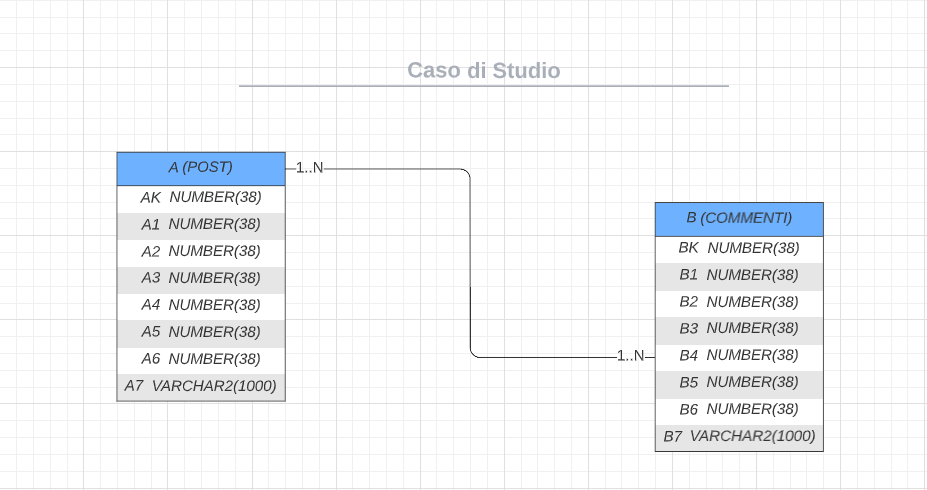
\includegraphics[scale=0.6]{Caso Studio.png}
\end{center}


\section{Modellazione dei dati}
Lorem ipsum dolor sit amet, consectetur adipiscing elit. Suspendisse et ex vehicula, interdum mi eu, auctor augue. Suspendisse vel sagittis urna. In vitae ligula ipsum. Vivamus mattis neque efficitur, gravida purus facilisis, rhoncus felis. Class aptent taciti sociosqu ad litora torquent per conubia nostra, per inceptos himenaeos. Nunc bibendum urna porta quam congue ornare. Fusce eget consequat libero. Donec varius justo vel libero malesuada, sit amet dignissim ex tincidunt. In pharetra vestibulum lacus quis laoreet. Donec vel laoreet ex, sed facilisis massa. Mauris commodo velit est. Maecenas non sem elementum, faucibus velit et, bibendum mi. Integer laoreet ex et eros accumsan, nec dapibus nisi vestibulum. Donec sed nunc quis mi gravida congue non vel tortor. Interdum et malesuada fames ac ante ipsum primis in faucibus.

Nullam non pharetra arcu. Donec eget velit elit. Pellentesque sed tortor sodales neque tristique rutrum. Vivamus et ex dolor. Vestibulum lacinia augue sit amet libero mattis pellentesque. In sed congue ante, quis tempus neque. Vestibulum semper eu sapien et vestibulum.

In ac erat ullamcorper, ultricies dolor sit amet, tempus neque. Pellentesque quam erat, ornare ac justo at, cursus luctus ex. Pellentesque at turpis blandit, elementum ex ac, fringilla nibh. Etiam et tincidunt lacus. Integer mattis mi sit amet faucibus rutrum. Sed at nisi commodo, ultricies purus a, tempus lacus. Mauris accumsan enim nisi, in tempor velit pharetra eu. Sed eu turpis et ante sagittis sodales. Duis a tellus id risus ultricies accumsan. Vestibulum bibendum in sapien sit amet rhoncus. Fusce aliquam, metus vel efficitur pulvinar, nibh lacus ultricies nisl, nec rhoncus elit ligula vitae risus. Mauris bibendum eget erat non rutrum. Curabitur in ligula eget lectus facilisis molestie sed sed neque. Vestibulum eu faucibus augue, a luctus augue. Nam lobortis massa non lorem condimentum vehicula. Aliquam efficitur cursus neque, efficitur placerat libero tincidunt non. Nullam.

\begin{center}
    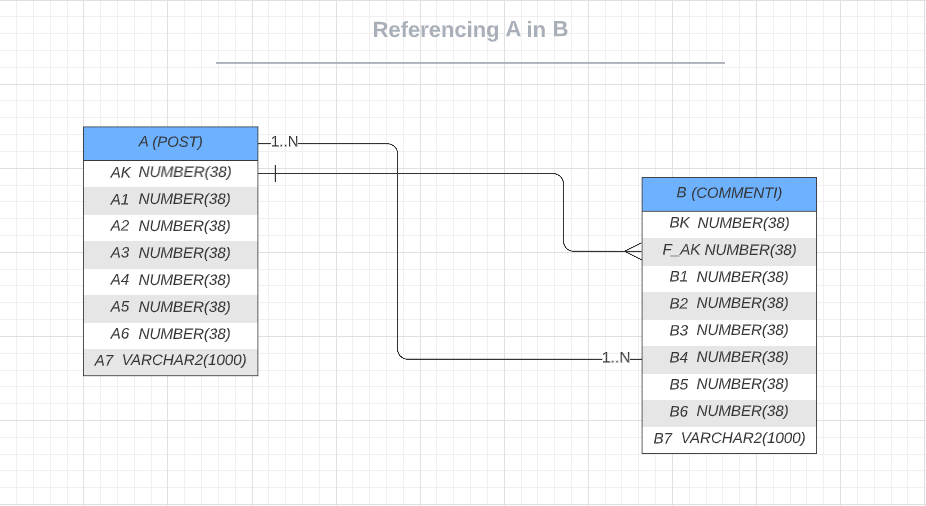
\includegraphics[scale=0.6]{refAB.png}
\end{center}

\begin{center}
    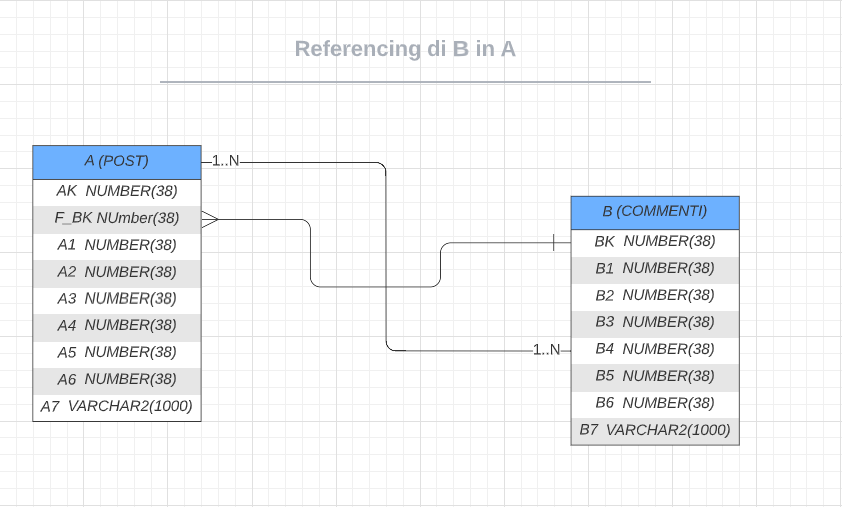
\includegraphics[scale=0.6]{refBA.png}
\end{center}

\begin{center}
    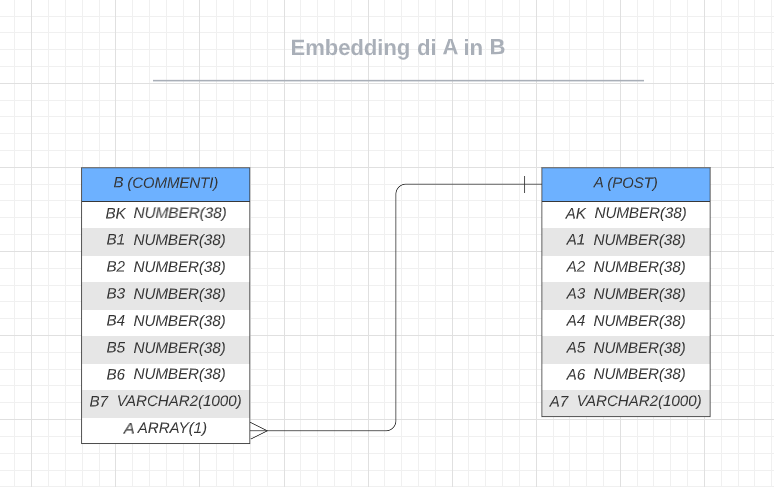
\includegraphics[scale=0.6]{embAB.png}
\end{center}

\begin{center}
    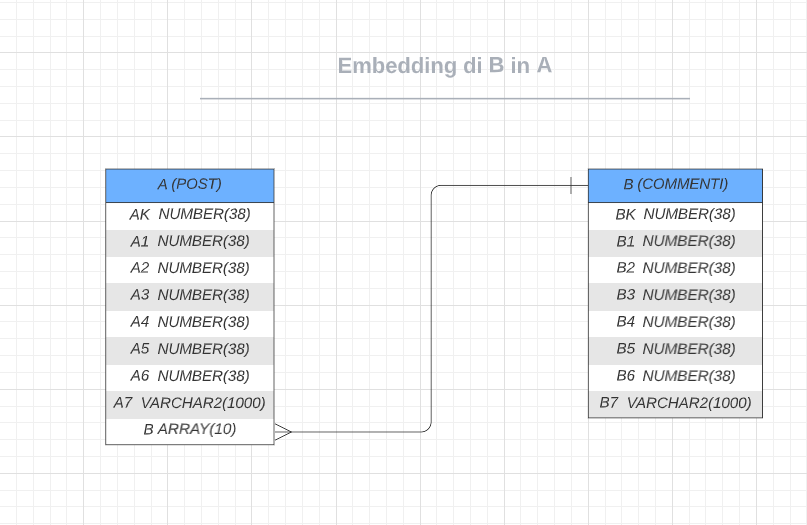
\includegraphics[scale=0.6]{embBA.png}
\end{center}

  \chapter{Costi}

\section{Calcolo dei costi}

La parte teorica di questo progetto si basa sulla stima di costi di esecuzione delle operazioni sulle differenti opzioni di organizzazione dei documenti, per calcolare cio' 
abbiamo bisogno di alcune formule che andro qui ad elencare:  

\subsection{NL}
    \begin{equation*}
        \begin{aligned}
        NL &=\floor*{\frac{NK * len(k) + NR * len(p)}{D * u}}
        \end{aligned}
        \end{equation*}
\subsection{g}
    \begin{equation*}
        \begin{aligned}
        g &=\ceil*{\frac{D - len(p)}{2 * (len(k) + len(p))}}
        \end{aligned}
        \end{equation*}
\subsection{h}
    \begin{equation*}
        \begin{aligned}
        \floor*{\log_{(2*g + 1)}{NL}} \leq h \leq \ceil*{\log_{(g + 1)}{\frac{NL}{2}}}
        \end{aligned}
        \end{equation*}
\subsection{NP}
    \begin{equation*}
        \begin{aligned}
        NP &=\floor*{\frac{NR * len(t)}{D * u}}
        \end{aligned}
        \end{equation*}
\subsection{Costo del nested loop}
In cui ho R relazione esterna e S relazione interna
\begin{itemize}
    \item senza predicato di selezione 
    \begin{equation*}
        \begin{aligned}
        NP_R + NR_R * NP_S
        \end{aligned}
        \end{equation*}
    \item con predicato di selezione 
    \begin{equation*}
        \begin{aligned}
            NP_R + (sel(pred) * NR_R) * costo(S)
        \end{aligned}
        \end{equation*}
\end{itemize}
\subsection{Indice clustered}
    \begin{equation*}
        \begin{aligned}
            Costo(S)&= (h -1) + \floor*{\frac{1}{NK} * NL} +  \floor*{sel(pred) * NP}
        \end{aligned}
        \end{equation*}
\subsection{Indice unclustered}
    \begin{equation*}
        \begin{aligned}
            Costo(S)&= (h -1) + \floor*{\frac{1}{NK} * NL} + 1 + \phi(\frac{NR}{NK}, NP)
        \end{aligned}
        \end{equation*}

\begin{center}
    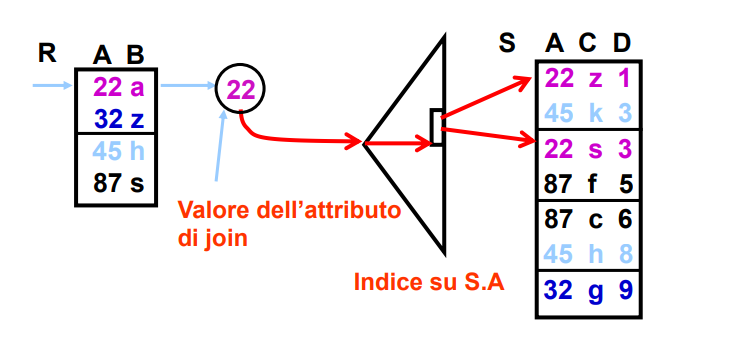
\includegraphics{nestedLoop.png}
\end{center}


\begin{center}
    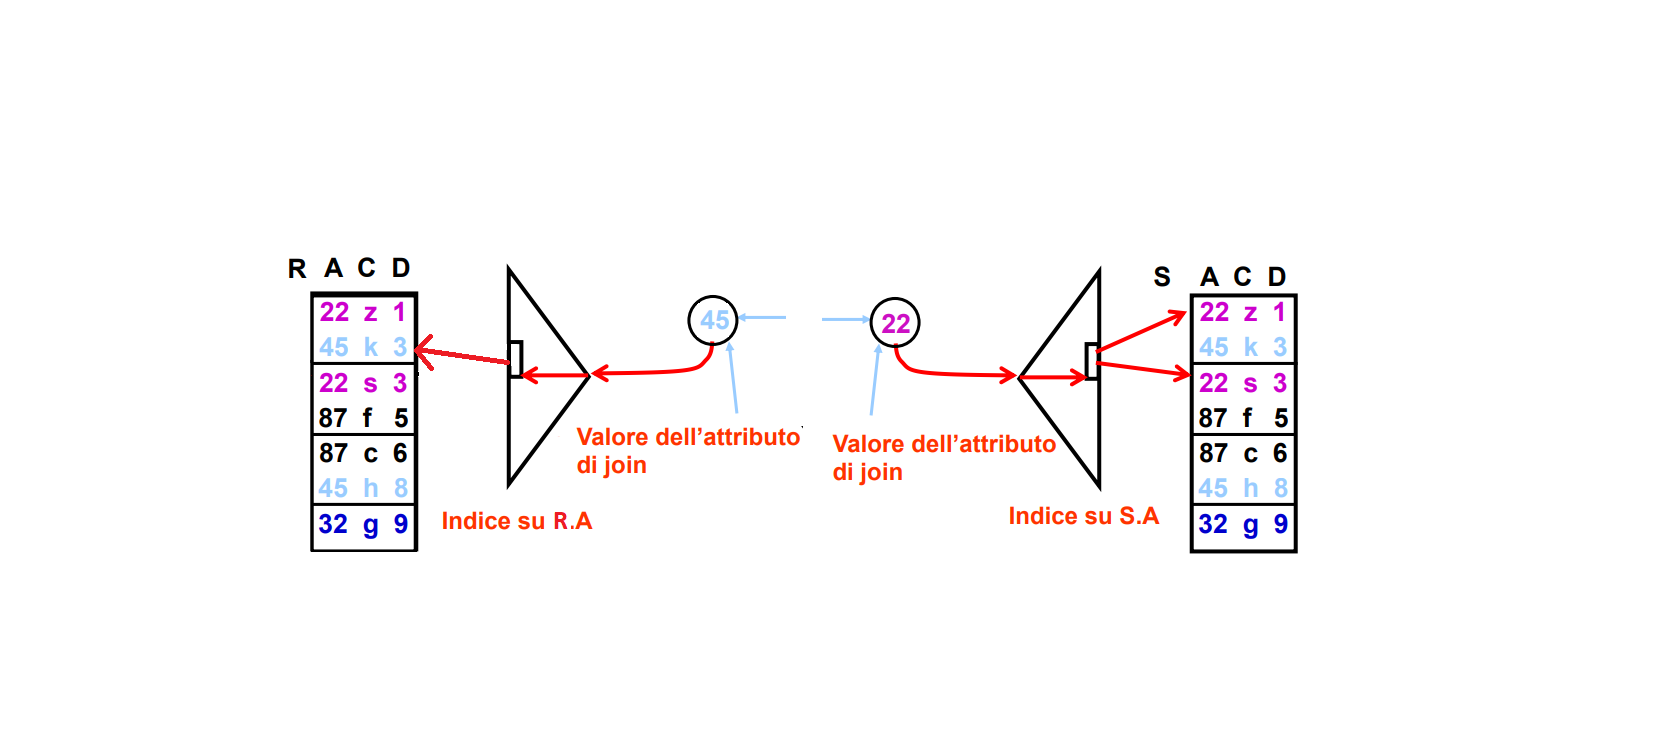
\includegraphics[scale=0.4]{nestedLoop 2 indici.png}
\end{center}
  \chapter{MongoDb}

\section{Caratteristiche}

MongoDb e' uno dei piu' diffusi database non relazionali orientato ai documenti, di tipo NoSQL,  utilizza documenti in un formato JSON al posto delle tipiche tabelle 
dei sistemi relazionali. Piu' precisamente MongoDb utilizza i BSON ossia JSON binari per rappresentare strutture dati semplici e array associativi (oggetti in MongoDb),
un BSON contiene una lista ordinata di elementi appartenenti ai seguenti tipi:

\begin{itemize}{}{}
    \item stringhe
    \item interi (32 o 64 bit)
    \item double (numeri a virgola mobile a 64 bit, standard IEEE 754)
    \item date (numeri interi in millisecondi dal'epoca Unix come riferimento, 1º gennaio 1970)
    \item byte array (dati binari)
    \item booleani (true e false)
    \item NULL
    \item oggetto BSON
    \item array BSON
    \item espressioni regolari
    \item codice JavaScript
\end{itemize}

\section{Organizzazione dei dati}

\subsection{Creazione collezioni}

Per poter originare i set di dati sui quali lavoriamo siamo partiti da 2 enormi file JSON generati al paragrafo ??????????? //TODO riguarda qua //
contenenti POST (A) e COMMENTI(B). Il paramentro \$out posto dopo la query ha creato una collezione a tuttli gli effetti sulla quale poter eseguire le query
all'interno della rete del container.

\subsubsection{Referencing}

Il referencing di A in B si ottiene facilmente proiettando gli attributi della collezione B, dato che contiene al suo interno la foreign Key di A.

\subsubsection{Referencing di A in B}

\begin{verbatim}
db.B.aggregate([
  {
    $project: {
      "_id" : "$BK",
      "BK" : "$BK",
      "AK" : "$FAK",
      "B1" : "$B1",   
      "B2" : "$B2",
      "B3" : "$B3",
      "B4" : "$B4",
      "B5" : "$B5",
      "B6" : "$B6",
      "B7" : "$B7"
    }
  },{
  $out : "referencing_A_in_B"
}
])
\end{verbatim}

Il referencing di B in A invece richiede un join, un' operazione piu' onerosa per la quale ho dovuto passare il parametro allowDiskUse=true per poter utilizzare
a pieno la memoria della macchina e quindi eseguire il join trovando di fatto le chiavi e aggiungendole all'array B che arrivera' a contenere 10 chivi BK per ogni 
AK dato che il rapporto e' di 1:10. 

\subsubsection{Referencing di B in A}

\begin{verbatim}
    
db.B.aggregate(
[
   {
      $group: {
        _id: {"AK" : "$FAK"}, "BK": {$addToSet : "$BK"}
      }
    },
    {
      $lookup: {
        from: 'Ap',
        localField: '_id.AK',
        foreignField: 'AK',
        as: 'AK'
      }
    },{
      $project : {"_id" : 0,"BK.FAK" : 0}
    },{
    $unwind: {
      path: "$AK",
    }},{
      $project : {
      "_id" : "$AK.AK",
      "AK" : "$AK.AK",
      "A1" : "$AK.A1", 
      "A2" : "$AK.A2", 
      "A3" : "$AK.A3", 
      "A4" : "$AK.A4",
      "A5" : "$AK.A5",
      "A6" : "$AK.A6",
      "A7" : "$AK.A7",
       "B" : "$BK"} 
    },{
      $out : "referencing_B_in_A"
    }
  ],{allowDiskUse:true}
)
\end{verbatim}

\subsubsection{Embedding}
Per l'embedding di documenti ho dovuto sempre eseguire dei join ma e' stato fondamentale poter aggiungere un intero documento all'interno di un'array tramite il parametro
\verb|$$ROOT| che ha permesso un operazione molto piu'veloce e compatta.

\subsubsection{Embedding di A in B}
 

\begin{verbatim}
db.B.aggregate(
  [
    {
      $lookup: {
        from: 'A',
        localField: 'FAK',
        foreignField: 'AK',
        as: 'A'
      }
    }
   ,{
     $project: {
       "FAK" : 0,
       "_id" : 0,
       "A._id" : 0
     }
   }
  ,{
    $project : {
      "_id" : "$BK",
      "B1" : 1,
      "B2" : 1,
      "B3" : 1,
      "B4" : 1,
      "B5" : 1,
      "B6" : 1,
      "B7" : 1,
      "A" : 1
    }
  }
  ,{
     $out : "embedding_A_in_B"
   }
  ]
)    
\end{verbatim}

\subsubsection{Embedding di B in A}

\begin{verbatim}
    db.B.aggregate(
  [
   {
      $group: {
        _id: {"AK" : "$FAK"}, "BK": {$addToSet : "$$ROOT"}
      }
    },
    {
      $lookup: {
        from: 'A',
        localField: '_id.AK',
        foreignField: 'AK',
        as: 'AK'
      }
    },{
      $project : {"_id" : 0,"BK.FAK" : 0}
    },{
    $unwind: {
      path: "$AK",
    }},{
      $project : {
        "_id" : "$AK.AK",
        "AK" : "$AK.AK", 
        "A1" : "$AK.A1", 
        "A2" : "$AK.A2", 
        "A3" : "$AK.A3", 
        "A4" : "$AK.A4",
        "A5" : "$AK.A5",
        "A6" : "$AK.A6",
        "A7" : "$AK.A7",
        "B" : "$BK"} 
    },{
        $project : { "A._id" : 0, "B._id" : 0}
    },{
        $out : "embedding_B_in_A"
   }
  ],{allowDiskUse:true}
)
\end{verbatim}

\subsection{Indici}

Gli indici per gli attributi sono stati creati attraverso uno script in JS che viene eseguito durante la creazione del container.

MongoDB utilizza, se non esplicitamente indicato, come strutture dati per gli indici dei B-tree. Dato che abbiamo scelto di adoperare l'embedding di interi documenti sono stati 
indicizzati anche gli attributi dei documenti "innestati" sui quali saranno esegeuite delle query, anche sulle foreign del referencing sono stati costruiti indici.

\begin{center}
  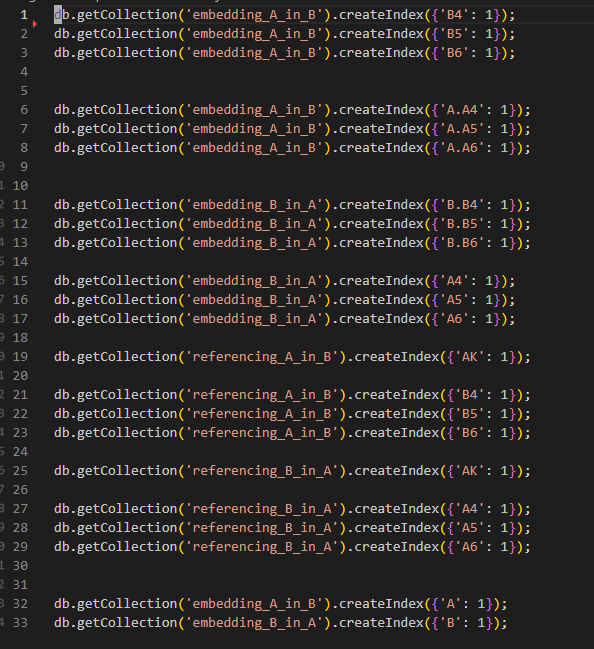
\includegraphics{../code/makeIndexes.png}
\end{center}

\begin{lstlisting}[caption=making indexes, style=customJs]
// indexes
db.getCollection('embedding_A_in_B').createIndex({'B4': 1});
db.getCollection('embedding_A_in_B').createIndex({'B5': 1});
db.getCollection('embedding_A_in_B').createIndex({'B6': 1});

// nested indexes
db.getCollection('embedding_A_in_B').createIndex({'A.A4': 1});
db.getCollection('embedding_A_in_B').createIndex({'A.A5': 1});
db.getCollection('embedding_A_in_B').createIndex({'A.A6': 1});

// indexes
db.getCollection('embedding_B_in_A').createIndex({'A4': 1});
db.getCollection('embedding_B_in_A').createIndex({'A5': 1});
db.getCollection('embedding_B_in_A').createIndex({'A6': 1});

// nested indexes
db.getCollection('embedding_B_in_A').createIndex({'B.B4': 1});
db.getCollection('embedding_B_in_A').createIndex({'B.B5': 1});
db.getCollection('embedding_B_in_A').createIndex({'B.B6': 1});

//FK
db.getCollection('referencing_A_in_B').createIndex({'AK': 1});               

// indexes
db.getCollection('referencing_A_in_B').createIndex({'B4': 1});
db.getCollection('referencing_A_in_B').createIndex({'B5': 1});
db.getCollection('referencing_A_in_B').createIndex({'B6': 1});

//FK
db.getCollection('referencing_B_in_A').createIndex({'AK': 1});               

// indexes
db.getCollection('referencing_B_in_A').createIndex({'A4': 1});
db.getCollection('referencing_B_in_A').createIndex({'A5': 1});
db.getCollection('referencing_B_in_A').createIndex({'A6': 1});

// array indexes
db.getCollection('embedding_A_in_B').createIndex({'A': 1});
db.getCollection('embedding_B_in_A').createIndex({'B': 1});
\end{lstlisting}

% \lstinputlisting[caption=making indexes, style=customJs]

  \chapter{Oracle}

\section{Introduzione}

Oracle e' una societa' che mette a disposizione numerosi prodotti, per la parte di confronto relazionale e' stato usato oracle SQL developer, un software opensource che 
mette a disposizione un software per poter lavorare con SQL su database di Oracle attraverso il JDK (java development kit).

\section{Raccolta dati}

\section{Organizzazione dei dati}

Utilizzando un sistema relazionale ci si e' dovuti limitare alla crezione di due collezioni distinte A (Post) e B(Commenti) sulle quali eseguire le query di selezione per poter
ottenere una stima dei costi su un modello relazionale che non utlizasse embedding e referencing.

Sono stati creati file .csv dei dati facilmente importabili in un database Oracle creato su un computer fisso, sui quali sono state effettuate alcune operazioni come la creazione di 
indici per specifici attributi e la limitazione della memoria cache del database locale. 

\begin{minted}[]{sql}
        -- Primary key per A

        alter table "SYS"."A" add constraint PK primary key("AK") 

        -- Primary key per B

        alter table "SYS"."B" add constraint PKB primary key("BK") 

        -- Aggiungere il constraint per FAK

        ALTER TABLE B
          ADD CONSTRAINT FK_A_constr FOREIGN KEY (FAK)     
              REFERENCES A(AK)
              ON DELETE CASCADE;

        -- Indici

        CREATE BITMAP INDEX A_A4_BITMAP ON A (A4 ASC);
        CREATE BITMAP INDEX A_A5_BITMAP ON A (A5 ASC);
        CREATE BITMAP INDEX A_A6_BITMAP ON A (A6 ASC);
        CREATE BITMAP INDEX B_B4_BITMAP ON B (B4 ASC);
        CREATE BITMAP INDEX B_B5_BITMAP ON B (B5 ASC);
        CREATE BITMAP INDEX B_B6_BITMAP ON B (B6 ASC);
        CREATE BITMAP INDEX B_FK_BITMAP ON B (FAK ASC);

        -- Ridurre la cache del client di sistema

        ALTER SYSTEM SET CLIENT_RESULT_CACHE_SIZE = 128M SCOPE=SPFILE;
 
\end{minted}


\section{Inserimento (CRUD: Creation)}


Oracle è un database relazionale, sul quale risulta semplice inserire una tupla all'interno di una tabella attraverso PL/SQL ma nel caso di una quantità
cospiqua di dati non è piu possibile utilizzare quel metodo che funziona nei piccoli numeri. Il software non riesce a completare quei task cosi ci si è 
appoggiati alla funzionalità di importazione da file, in particolare si è adattato il dataset ad essere un file di tipo .csv che è stato facilmente 
inserito all'interno dell'istanza del database.

\begin{center}
    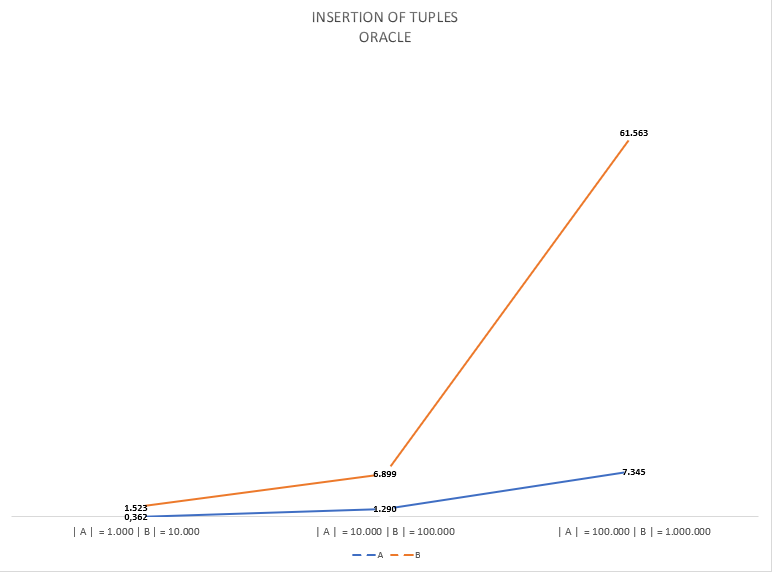
\includegraphics[scale=0.8]{InsertionOracle.png}
\end{center}

//TODO server section


\section{Selezione (CRUD: Read)}

Per poter eseguire le query di selezione e' stato utilizzato uno script in python che utilizza il modulo \verb|cx_Oracle| per poter creare una connessione 
al database locale ed effettuare un numero arbitrario di query, ogni query effettuata riporta un piano di esecuzione visionabile nell'apposito file 
.sql. Dopo che la connessione viene confermata, si procede a creare 
un cursore con il quale si andranno ad eseguire query articolate come segue:

\begin{minted}[]{sql}
        EXPLAIN PLAN FOR SELECT * FROM A WHERE A6 = 612;
        SELECT PLAN_TABLE_OUTPUT FROM TABLE(DBMS_XPLAN.DISPLAY());
\end{minted}

Che provvedono ad esegure una query e scrivere una riga all'interno del \verb|PLAN_TABLE_OUTPUT| che poi verra letta e salvata 
in un file, per poter avere una copia del piano di esecuzione di ciascuna query.

\begin{table}[!ht]
    \centering
    \begin{tabular}{|l|l|l|}
    \hline
        ~ & A & B \\ \hline
        A0 & 15 & ~ \\ \hline
        A1 & 47 & ~ \\ \hline
        A2 & 17 & ~ \\ \hline
        A3 & 6 & ~ \\ \hline
        A4 & 4 & ~ \\ \hline
        A5 & 1 & ~ \\ \hline
        A6 & 1 & ~ \\ \hline
        B0 & ~ & 7 \\ \hline
        B1 & ~ & 295 \\ \hline
        B2 & ~ & 10 \\ \hline
        B3 & ~ & 5 \\ \hline
        B4 & ~ & 3 \\ \hline
        B5 & ~ & 5 \\ \hline
        B6 & ~ & 1 \\ \hline
        A0j & 5 & ~ \\ \hline
        A1j & 15 & ~ \\ \hline
        A2j & 3 & ~ \\ \hline
        A3j & 4 & ~ \\ \hline
        A4j & 3 & ~ \\ \hline
        A5j & 2 & ~ \\ \hline
        A6j & 3 & ~ \\ \hline
        B0j & ~ & 4 \\ \hline
        B1j & ~ & 524 \\ \hline
        B2j & ~ & 10 \\ \hline
        B3j & ~ & 937 \\ \hline
        B4j & ~ & 2 \\ \hline
        B5j & ~ & 5 \\ \hline
        B6j & ~ & 797 \\ \hline
    \end{tabular}
\end{table}


\section{Aggiornamento (CRUD: Update)}

Le query di aggiornamento dei dati hanno prodotto i seguenti risultati 
  \chapter{CouchDb}

\section{Raccolta dati}
Lorem ipsum dolor sit amet, consectetur adipiscing elit. Suspendisse et ex vehicula, interdum mi eu, auctor augue. Suspendisse vel sagittis urna. In vitae ligula ipsum. Vivamus mattis neque efficitur, gravida purus facilisis, rhoncus felis. Class aptent taciti sociosqu ad litora torquent per conubia nostra, per inceptos himenaeos. Nunc bibendum urna porta quam congue ornare. Fusce eget consequat libero. Donec varius justo vel libero malesuada, sit amet dignissim ex tincidunt. In pharetra vestibulum lacus quis laoreet. Donec vel laoreet ex, sed facilisis massa. Mauris commodo velit est. Maecenas non sem elementum, faucibus velit et, bibendum mi. Integer laoreet ex et eros accumsan, nec dapibus nisi vestibulum. Donec sed nunc quis mi gravida congue non vel tortor. Interdum et malesuada fames ac ante ipsum primis in faucibus.

Nullam non pharetra arcu. Donec eget velit elit. Pellentesque sed tortor sodales neque tristique rutrum. Vivamus et ex dolor. Vestibulum lacinia augue sit amet libero mattis pellentesque. In sed congue ante, quis tempus neque. Vestibulum semper eu sapien et vestibulum.

In ac erat ullamcorper, ultricies dolor sit amet, tempus neque. Pellentesque quam erat, ornare ac justo at, cursus luctus ex. Pellentesque at turpis blandit, elementum ex ac, fringilla nibh. Etiam et tincidunt lacus. Integer mattis mi sit amet faucibus rutrum. Sed at nisi commodo, ultricies purus a, tempus lacus. Mauris accumsan enim nisi, in tempor velit pharetra eu. Sed eu turpis et ante sagittis sodales. Duis a tellus id risus ultricies accumsan. Vestibulum bibendum in sapien sit amet rhoncus. Fusce aliquam, metus vel efficitur pulvinar, nibh lacus ultricies nisl, nec rhoncus elit ligula vitae risus. Mauris bibendum eget erat non rutrum. Curabitur in ligula eget lectus facilisis molestie sed sed neque. Vestibulum eu faucibus augue, a luctus augue. Nam lobortis massa non lorem condimentum vehicula. Aliquam efficitur cursus neque, efficitur placerat libero tincidunt non. Nullam.

  \mainmatter{}
  \pagenumbering{arabic}
  \pagestyle{headings}
  Minimo documento
  \appendix
  \begin{appendices}
  Appendice
\end{appendices}


  \backmatter{}
  \nocite{*}            % aggiunge tutti i riferimenti nel .bib (anche non citati)
\printbibliography[%  % produce la bibliografia
  heading=bibintoc    % inserisce il titolo nell'indice generale
]

  Ringraziamenti


\end{document}
